\documentclass[../main.tex]{subfiles}
\graphicspath{{\subfix{../images/}}}

\begin{document}
This section contains a formal analysis of the system performed with the declarative language Alloy. It is based on the description of the model of the system with its components and the interactions between them, with a particular focus on the constraints of the system. The validity of the 
\\
\\


\subsection{Alloy code}

\begin{lstlisting}
//email is an identification for all the users
sig Email{}
//password for the user
sig Password{}
//lincence number of a driver
sig LicenceId{}
//plate number of a vehicle
sig PlateNumber{}

//price of energy or of 
sig Price{}
//date for reservation and charging process
sig Date{}
//time slot for reservation
sig TimeSlot{}
//location of charging station
sig Location{}
//energy supplied by charging station
sig Energy{}


//charging type of a socket in the charging station
abstract sig ChargeType{}
one sig SLOW extends ChargeType{}
one sig FAST extends ChargeType{}
one sig RAPID extends ChargeType{}

//boolean
abstract sig Bool {}
one sig TRUE extends Bool {} 
one sig FALSE extends Bool {}

//all users of e-Mall
abstract sig User {
	email: one Email,
	password: one Password
}

//driver: user of electric vehicles
sig Driver extends User {
	licence_id: one LicenceId
} 

//operator: charging station administrator working for a CPO
sig Operator extends User {
}

//CPO: company which owns and manages charging stations
sig CPO{
	operators: some Operator
}

//vehicle that belongs to a driver
sig Vehicle {
	plate_number: one PlateNumber,
	battery_status: one Int,
    	drivers: some Driver
}{
	battery_status >= 0
}

//charging stations where drivers go to charge their vehicles
sig ChargingStation {
	location: one Location,
	number_socket: one Int,
	sockets: some Socket,
	energy_price: one Price,
	cpo: one CPO
}{	
	number_socket = #sockets
}

//socket used for charging a vehicle
sig Socket {
	available: one Bool,
	type: one ChargeType,
	amount_power: one Int,
	energy: one Energy
}{
	amount_power >= 0
}

//offer set by a charging station with expire time
sig Offer {
	from_date: one Date,
	to_date: one Date,
	price: one Price,
	cstation: one ChargingStation
} 

//charging process of charging a vehicle
sig ChargingProcess{
	vehicle: one Vehicle,
	date: one Date,
	estimated_time: one Int,
	price: one Price,
	reservation: one Reservation,
	socket: one Socket
} {
	estimated_time >= 0 and vehicle = reservation.vehicle and date = reservation.date and socket = reservation.socket
}

//a reservation by a driver to charge his vehicle
sig Reservation{
	vehicle: one Vehicle,
	date: one Date,
	time_slot: one TimeSlot,
	offer: lone Offer,
	socket: one Socket,
	charge_quantity: one Int
} { 
	charge_quantity > 0 and socket in offer.cstation.sockets
}

/* fact */
//all the operators must belong to at least one CPO
fact allOperatorBelongsToCPO {
	all op : Operator |
	(one cpo: CPO | op in cpo.operators)
}

//all the sockets must belong to at least a charging station
fact allSocketBelongsToCS {
	all s: Socket |
	(one cs: ChargingStation | s in cs.sockets)
}

//one socket must not have different reservations at the same time
fact uniqueTimeSlotForSameSocket	{
	no disjoint r1, r2: Reservation | r1.time_slot = r2.time_slot and r1.socket = r2.socket and r1.date = r2.date
}

//a vehicle must have one and only one reservation on the same date and in the same time slot
fact uniqueReservationForSameVehicle {
	no disjoint r1, r2: Reservation | r1.time_slot = r2.time_slot and r1.vehicle = r2.vehicle and r1.date = r2.date
}

//there are no different charging stations in the same location
fact uniqueLocation {
    no disjoint cs1, cs2 : ChargingStation | cs1.location = cs2.location
}

//a reservation must have one and only one charging process
fact uniqueReservationForACProcess {
	no disjoint cp1, cp2 : ChargingProcess | cp1.reservation = cp2.reservation 
}

//every identification of licence ID is associated to one and only one driver
fact allLicenceIdBelongsToDriver{
	all li:LicenceId | one d:Driver | li = d.licence_id
}

//every plate number belongs to one and only one vehicle
fact allPlateNumberBelongsToVehicle{
	all pn: PlateNumber | one v:Vehicle | pn = v.plate_number
}

//every email belongs to one and only one user
fact allEmailBelongsToUser{
	all e: Email | one u: User | e = u.email
}


/* pred */

//add a driver to an vehicle
pred addDriver [v1, v2: Vehicle, d: Driver] {
	v2.drivers =  v1.drivers + d
}

//del a driver to an vehicle
pred delDriver [v1, v2: Vehicle, d: Driver] {
	v2.drivers =  v1.drivers - d
}


/* assert */

//checking for operation correctness
assert delUndoesAddDriverToVehicle {
	all d: Driver, v1, v2, v3: Vehicle |
	(not (u in v1.drivers) implies
		(addDriver[v1, v2, u] and delDriver[v2, v3, u]
		implies
		v1.drivers =  v3.drivers
	))
}
check delUndoesAddDriverToVehicle

//emails of users are unique
assert UniqueEmail {
	 no disjoint u1, u2: User | u1.email = u2.email 
}
check UniqueEmail

//every vehicle has at least one driver
assert everyVehicleHasADriver{
	all v: Vehicle |
	(some d: Driver |  d in v.drivers)
}
check everyVehicleHasADriver

//every charging station has at least one socket
assert everyChargingStationHasSocket{
	all cs: ChargingStation |
	(some s: Socket | s in cs.sockets)
}
check everyChargingStationHasSocket

//identifiers are all unique
assert UniqueIdentifier{
	 no disjoint d1, d2: Driver| d1.licence_id = d2.licence_id and
	 no disjoint v1, v2: Vehicle | v1.plate_number = v2.plate_number
}
check UniqueIdentifier

//every charging process must have one and only one reservation
assert everyChargingProcessHasReservation{
	all cp: ChargingProcess |
	(one r: Reservation | cp.reservation = r)
}
check everyChargingProcessHasReservation

//every charging station has at least one operator
assert everyCStaionHasOperator{
	all cs: ChargingStation|
	(some o: Operator | o in cs.cpo.operators)		
}
check everyCStaionHasOperator

//all offer must be created by one and only one charging station
assert allOfferBelongsToCS{
	all of: Offer |
	(one cs: ChargingStation | of.cstation = cs)
}
check allOfferBelongsToCS


pred world {
  	#Vehicle>0
	#Socket>0
	#Offer>0
	#Reservation = 1
	#ChargingProcess>0
	#ChargingStation>0
	#Operator = 2
}ß
run world for 3


\end{lstlisting}


\subsection{Generated model}
It is shown below a simple scenario, where a charging process is presented. In this instance there are 3 users: 1 driver and 2 operators. The vehicle of the driver is charged at a charging station after reservation. An offer is also applied on the charging. The two operators work for the same CPO, which manage the charging station.

\begin{figure}[H]
    \centering
    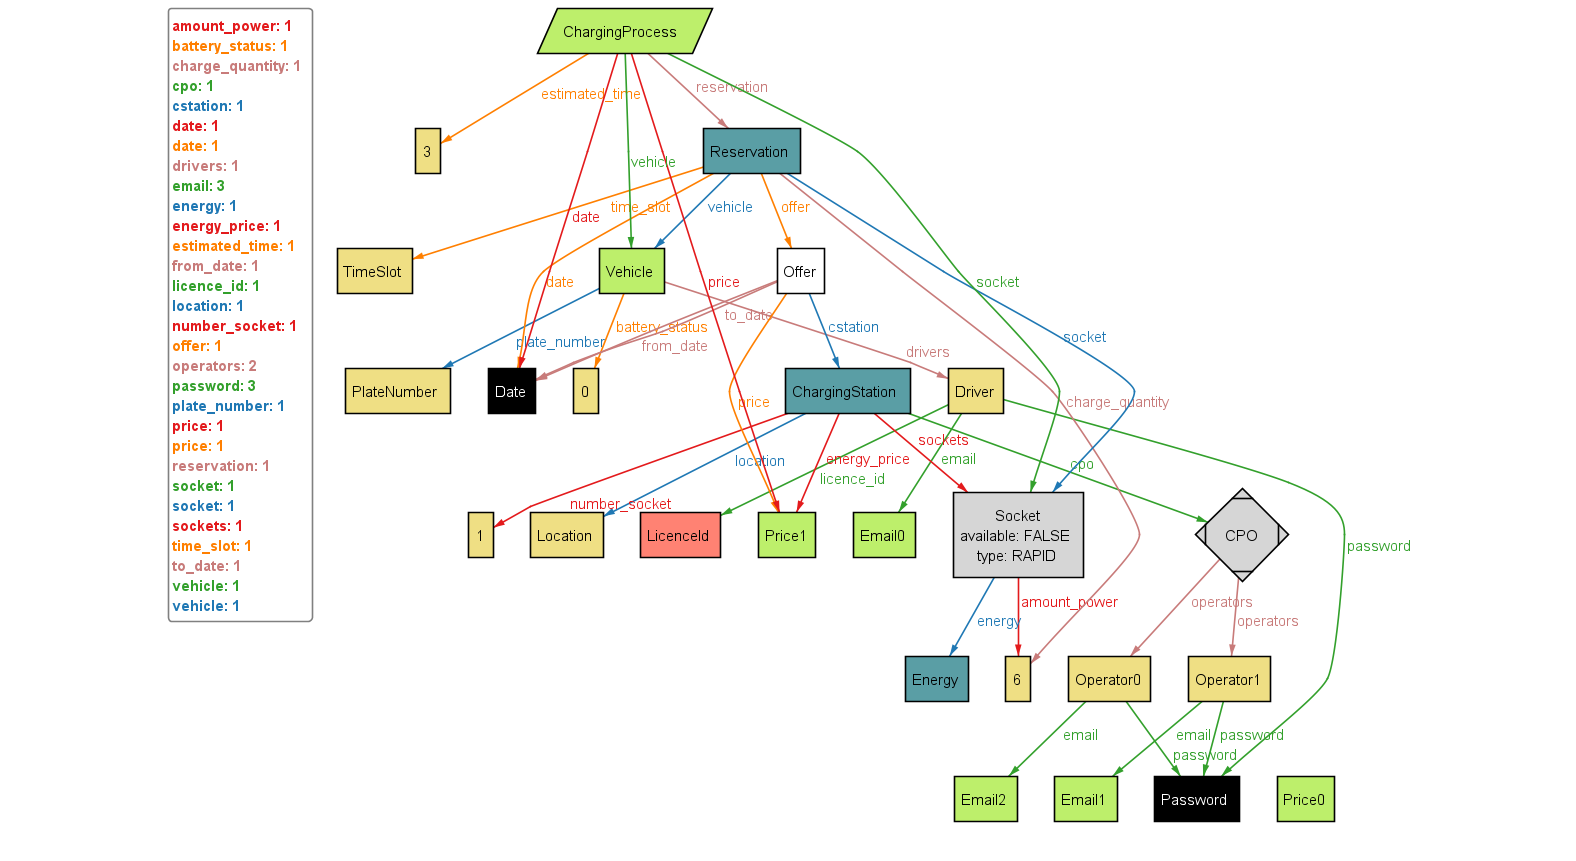
\includegraphics[width=\textwidth]{images/alloyworld.png}
    \caption{Generated Alloy model}
    \label{fig:class}
\end{figure}

\\
Moreover, this instance satisfies all the following constraints:

\begin{itemize}
    \item Every vehicle has a driver
    \item Every socket has a charging station
    \item All identifiers are unique
    \item Every charging process has a reservation
    \item Every charging station has at least an operator
\end{itemize}

\begin{figure}[H]
    \centering
    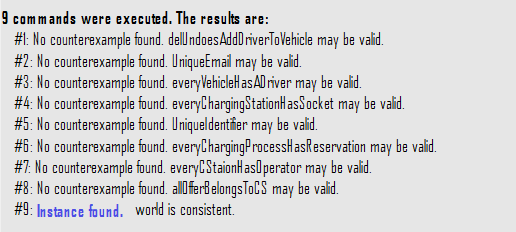
\includegraphics[width=0.8\textwidth]{images/constraints.png}
    \caption{Validation of the Alloy model}
    \label{fig:class}
\end{figure}


\end{document}